\documentclass[10pt,a4paper]{article}

\usepackage{polski}
\usepackage[utf8]{inputenc}
\usepackage[polish]{babel}
\usepackage{hhline}
\usepackage{pgfplots}
\usepackage{multicol}
%\usepackage{slashbox}
\usepackage{graphicx}
\usepackage{caption}
\usepackage{subcaption}
\usepackage{colortbl}
\usepackage{geometry}
\usepackage{listings}
\usepackage{mathtools}
\DeclarePairedDelimiter\ceil{\lceil}{\rceil}
\DeclarePairedDelimiter\floor{\lfloor}{\rfloor}
\geometry{a4paper, total={170mm,257mm}, left=20mm, top=20mm }
\lstset
{
    language=C++,
    basicstyle=\footnotesize,
    numbers=left,
    stepnumber=1,
    showstringspaces=false,
    tabsize=1,
    breaklines=true,
    breakatwhitespace=false,
}
\author{Sebastian Maciejewski 132275 i Jan Techner 132332\\
grupa I1, zajęcia we wtorki o 15:10, tygodnie nieparzyste,\\
email: maciejewski.torun@gmail.com}
\title{Porównywanie efektywności metod mnożenia macierzy}
\date{30 kwietnia 2019}
\setlength{\parindent}{0pt}
\newcommand{\forceindent}{\leavevmode{\parindent=3em\indent}}
\begin{document}
\maketitle
\section{Wstęp}
Sprawozdanie dotyczy zadania w wariancie 22. - porównywanie efektywności metod
mnożenia macierzy:\\
- dla 3 pętli kolejność jki, podział pracy przed 1. pętlą\\
- dla 6 pętli kolejność pętli zewnętrznych ijk, wewnętrznych iijjkk,
podział pracy przed 4. pętlą\\
\\
Wszystkie pomiary zostały wykonane na komputerach laboratoryjnych w sali 2.7.6.
\section{Analiza przygotowania eksperymentu}
\subsection{Kod wykorzystywany przy pomiarach}
Kod, którego używaliśmy w eksperymencie został tak podzielony, aby cała
logika przetwarzania znajdowała się w pojedynczej funkcji. Poniżej prezentowany
jest kod tylko tych funkcji - generowanie macierzy i wypełnianie jej
losowymi liczbami, liczenie czasu i wypisywanie wyników działają w ten
sam sposób dla wszystkich wariantów przetwarzania.
\subsubsection{Metoda 3 pętli - równolegle}
\begin{lstlisting}
    void multiply_matrices_JKI()
    {
    #pragma omp parallel for 
        for (int j = 0; j < COLUMNS; j++)
            for (int k = 0; k < COLUMNS; k++)
                for (int i = 0; i < ROWS; i++)
                    matrix_r[i][j] += matrix_a[i][k] * matrix_b[k][j];
    }
\end{lstlisting}

\subsubsection{Metoda 3 pętli - sekwencyjnie}
\begin{lstlisting}
    void multiply_matrices_IKJ_sequentially() 
    {
        for (int i = 0; i < ROWS; i++)
            for (int k = 0; k < COLUMNS; k++)   
                for (int j = 0; j < COLUMNS; j++)
                    matrix_r[i][j] += matrix_a[i][k] * matrix_b[k][j];
    }
\end{lstlisting}

\subsubsection{Metoda 6 pętli - równolegle}
\begin{lstlisting}
    void multiply_matrices_IJK_IIJJKK()
    {
        int r = 10;
        for (int i = 0; i < ROWS; i += r)
            for (int j = 0; j < COLUMNS; j += r)
                for (int k = 0; k < COLUMNS; k += r)
    #pragma omp parallel for
                    for (int ii = i; ii < i + r; ii++)
                        for (int jj = j; jj < j + r; jj++)
                            for (int kk = k; kk < k + r; kk++)
                                matrix_r[ii][jj] += matrix_a[ii][kk] * matrix_b[kk][jj];
    }
\end{lstlisting}
\newpage

\subsection{Analiza podziału pracy na wątki}
\subsubsection{Dyrektywy OpenMP}
W naszym kodzie używamy dyrektyw 'pragma omp parallel for', które sprawiają, że iteracje pętli
będą wykonane w sposób równoległy przez kilka wątków. Każdy z wątków wykona jednakowy zakres
iteracji, w naszym wypadku, przy podziale na 4 wątki, pierwszy wątek wykona pierwszą $\frac{1}{4}$
operacji, drugi kolejną itd. Dopiero po zakończeniu przetwarzania przez wszystkie wątki następuje
synchronizacja i przejście dalej - do zakończenia pomiaru czasu.

\subsubsection{Analiza ryzyka wystąpienia wyścigu i zjawiska false sharingu}

\subsubsection*{Wyścig}

Zjawisko wyścigu, czyli równoległa modyfikacja tej samej zmiennej przez różne procesy, nie
występuje w naszym kodzie.\\
Aby się o tym przekonać wystarczy zwrócić na to, że w naszym przypadku,
w równoległym przetwarzaniu dla 3 pętli mamy zapis do $matrix\_r[i][j]$, gdzie wartości $j$ są
dzielone pomiędzy procesy z powodu wystąpienia dyrektywy 'parallel for' przed pętlą odpowiedzialną
za inkrementację licznika kolumn $j$ (2.1.1, linijki od 3 do 7). Co za tym idzie każdy proces zawsze zapisuje do innej kolumny
niż pozostałe, więc zjawisko wyścigu nie występuje w tym przypadku.\\
Podobna sytuacja występuje przy 6 pętlach - każdy proces zapisuje do osobnego wiersza z powodu
wystąpienia dyrektywy 'parallel for' przed pętlą odpowiedzialną za inkrementację zmiennej $ii$
(2.1.3, linijki od 7 do 11) - w tym przypadku również nie dojdzie do wyścigu.

\subsubsection*{False sharing}
Inaczej sytuacja ma się w przypadku zjawiska false sharingu. False sharing występuje wtedy, gdy
różne procesy zapisują zmienne znajdujące się w tej samej linii pamięci - wówczas kopie linii
w pamięciach podręcznych innych procesów stają się nieaktualne i dany proces musi ponownie pobrać
linię z pamięci aby zapewnić spójność pamięci podręcznej. To zajmuje czas, więc takie zjawisko
jest nieporządane, gdyż wpływa negatywnie na efektywność przetwarzania.\\
Długość linii pamięci w systemach, na których wykonywane były pomiary to 64B, zatem w każdej
linii pamięci mieści się 16 zmiennych typu float, używanych prez nas w obliczeniach. Rozmiary
instancji w naszych pomiarach były $\geq 400$. Mając to na uwadze, możemy się zająć analizą ryzyka
wystąpienia zjawiska false sharingu.\\

W wersji przetwarzania równolegle dla 3 pętli mamy do czynienia z podziałem pracy przed 1. pętlą, $j$,
która odpowiada za licznik kolumn.
Z uwagi na to, iż każdy z procesów zapisuje dane jedynie do swojej kolumny macierzy wynikowej,
zjawisko false sharingu nie wystąpi gdyż szerokość zbioru kolumn przetwarzanych przez jeden wątek jest
znacznie większa od długości jednej linii pamięci - dla instancji o wielkości 400, każdy wątek będzie
zapisywał dane do zbioru 100 kolumn, gdzie w jednym wierszu takiego zbioru zmieści się prawie 7 całych linii pamięci. \\
Jedynym miejscem, w którym to zjawisko może wystapić są brzegi zbiorów kolumn przetwarzanych przez wątki, kiedy linia pamięci
zawiera elementy wiersza należące do zbioru kolumn dwóch różnych wątków. Jednakże biorąc pod uwagę to, że wątki przetwarzają kolumny
sekwencyjnie, przesuwając się w lewo (zgodnie ze zmienna $j$), nawet jeżeli linia pamięci zawierająca ostatnie elementy zbioru kolumn przetwarzanych
przez wątek będzie zawierała elementy z następnego zbioru innego wątku, to te elementy już zostały przez ten wątek zapisane i linia pamięci zawierająca
te elementy została już zastąpiona przez nową linię, zawierającą elementy dalej na lewo w macierzy C.  \\

Natomiast w wersji 6-pętlowej zjawisko false-sharingu nie występuje, ponieważ każdy wątek zapisuje dane do swojego
zbioru wierszy fragmentu $r \times r$ macierzy C i i nie ma możliwości, żeby linia pamięci zawierała elementy wierszy przetwarzanych przez
dwa różne wątki.

\newpage

\subsubsection{Podział przetwarzania w metodzie 3-pętlowej}
\begin{figure}[h]
	\centering
	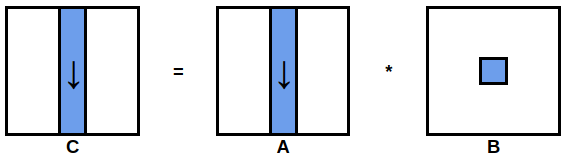
\includegraphics[width=0.5\textwidth]{3loops1.png}
	\caption{Obszar danych dla jednej wewnętrznej pętli $i$}
\end{figure}

Każdy wątek przy przechodzeniu ostatniej pętli odwołuje się do jednej kolumny macierzy wynikowej C (odwołanie następuje do elementu
$matrix\_r[i][j]$, gdzie zmianna $j$ jest stała dla ostatniej pętli), analogicznie dla macierzy A (w tym przypadku dla elementu $matrix\_a[i][k]$
nie zmienia się zmienna $k$). Przy przechodzeniu ostatniej pętli dla macierzy B, obie zmienne określające element $matrix\_b[k][j]$ są stałe, więc
wątki odwołują się tylko do jednego elementu macierzy B.

\begin{figure}[h]
	\centering
	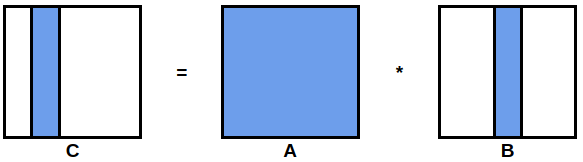
\includegraphics[width=0.5\textwidth]{3loops2.png}
	\caption{Obszar danych dla dwóch wewnętrznych pętli $k$ i $i$}
\end{figure}

Dla dwóch pętli każdy wątek przetwarza $k$ razy tą samą kolumnę macierzy C, co w przypadku jednej pętli, wszystkie kolumny
macierzy A oraz wszystkie elementy z $j$-tej kolumny macierzy C (zmienna $j$ jest cały czas stała).\\

Rozważając wszystkie pętle i podział pracy między wątkami, każdy wątek będzie po kolei przetwarzał kolejne kolumny macierzy C (wyznaczane przez
zmienną $j$), odpowiadające im kolumny macierzy B oraz każdorazowo całą macierz A.

\newpage

\subsubsection{Podział przetwarzania w metodzie 6-pętlowej}

\begin{figure}[h]
	\centering
	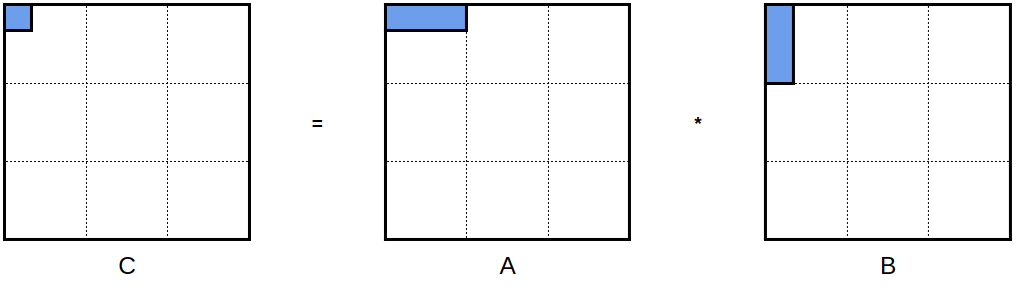
\includegraphics[width=0.5\textwidth]{6loops1.png}
	\caption{Obszar danych dla pętli $kk$}
\end{figure}

Przy przetwarzaniu ostatniej wewnętrznej pętli każdy wątek przetwarza jeden element macierzy C (zmienia się tylko zmienna $kk$, a odwołania następują do
elementu $matrix\_r[ii][jj]$), jeden cały wiersz o szerokości $r$ macierzy A (zmienna $ii$ pozostaje stała przy odwoływaniu się do elementu $matrix\_a[ii][kk]$) oraz
do jednej kolumny o wysokości $r$ macierzy B (przy odwoływaniu się do elementu $matrix\_b[kk][jj]$ zmienna $jj$ pozostaje stała).

\begin{figure}[h]
	\centering
	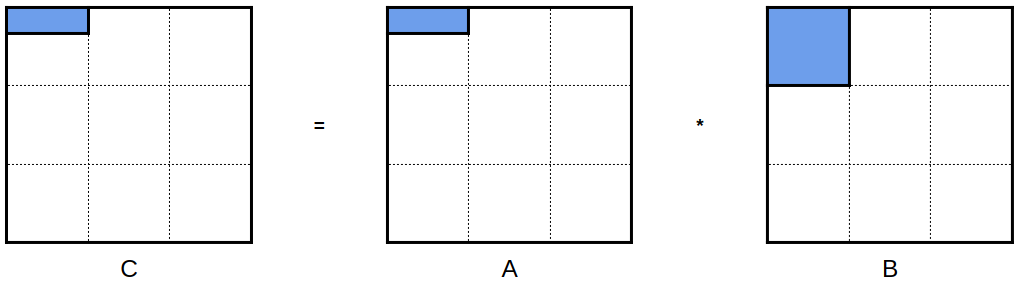
\includegraphics[width=0.5\textwidth]{6loops2.png}
	\caption{Obszar danych dla pętli $jj$, $kk$}
\end{figure}

Rozpatrując dwie pętle wewnętrzne, zmieniają się zmienne $jj$ i $kk$, czyli przy przetwarzaniu macierzy C zmieniane będą elementy z jednego wiersza
o szerokości $r$, $r$-krotnie przetwarzany będzie wiersz o szerokości $r$ macierzy A oraz wszystkie elementy fragmentu $r \times r$ macierzy B.

\begin{figure}[h]
	\centering
	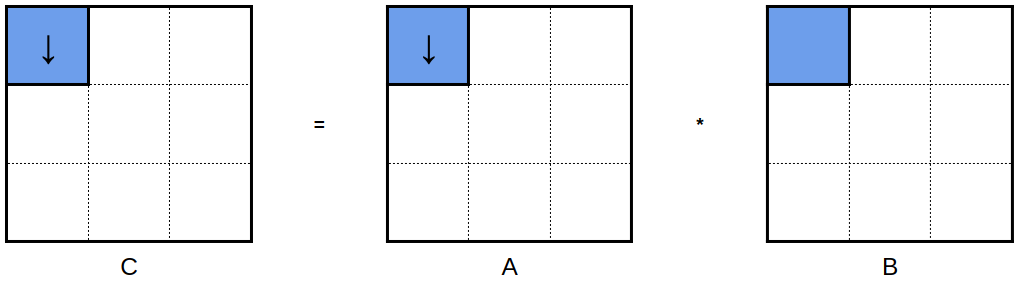
\includegraphics[width=0.5\textwidth]{6loops3.png}
	\caption{Obszar danych dla pętli $ii$, $jj$, $kk$}
\end{figure}

Dla 3 pętli wewnętrznych zmieniają się już wszystkie zmienne $ii$, $jj$ i $kk$, więc przetworzone zostaną wszystkie wiersze fragmentu $r \times r$
macierzy wynikowej C (odpowiada za to zmienna $ii$), wszystkie wiersze odpowiadającego fragmentu macierzy A oraz $r$ - krotnie przetworzone zostaną
wszystkie elementy fragmenu $r \times r$ macierzy B. \\

Podział pracy w naszym przypadku odbywa się przed pętlą $ii$, więc każdy wątek będzie przetwarzał grupę wierszy z fragmentu $r \times r$ macierzy C,
odpowiadający mu fragment macierzy A oraz wielkrotnie cały fragment $r \times r$ macierzy B.

\newpage

\subsection{Analiza lokalności czasowej}
Znaczącym czynnikiem mającym wpływ na efektywność przetwarzania jest czas dostępu do
danych. Ten czas jest znacznie krótszy przy dostępie podręczniej pamięci procesora niż
przy konieczności odwołania się do pamięci RAM. Bardzo ograniczona pojemność pamięci
podręcznej sprawia, że kod powinien być pisany w taki sposób, aby maksymalizować
wykorzystanie danych już załadowancyh do pamięci podręcznej i minimalizować ilość
odczytów z RAM. Przetwarzanie jest efektywne wtedy, gdy kod charakteryzuje się
czasową lokalnością odwołań do pamięci, czyli wielokrotnym wykorzystaniem danych załadowanych
do pamięci podręcznej zanim zostaną zastąpione innymi danymi odczytanymi z RAM.\\
Zakładamy, że rozmiar pamięci podręcznej procesora, na którym przeprowadzane są
obliczenia to 6 MB. Jest to pojemność pamięci L3 (L2 nie jest tu brane pod uwagę,
ponieważ część danych obecnych w niej pokrywa się z danymi w L3). Również pamięć L1
jest przy tym założeniu pomijana, ponieważ jej pojemność jest tak mała, że jej uwzględnianie
nie miało by znaczącego wpływu na obliczane wielkośći instancji.\\
Przy obliczeniach zakładamy, że 1 MB = 1000 KB = 1000000 B, przy czym pojedyncza zmienna typu
float, z których korzystamy, ma rozmiar 4 B.\\
\\
Dla metody \textbf{3 pętli} wzór, którego używamy do obliczania rozmiaru instancji, dla której
będzie zachowana lokalność czasowa to:
\begin{equation}
	n^2 * 4B + 2 * n * 64B \leq \frac{6000000B}{4}
\end{equation}
przy czym $n$ to rozmiar instancji.\\\\
Warunek zachowania lokalności czasowej będzie spełniony jeżeli pamięć podręczna pomieści:
\begin{enumerate} \itemsep0pt
	\item[a)] jedną kolumnę macierzy C (zajmowana pamięć wyniesie $n * 64B$, ponieważ macierz jest w pamięci
	      przechowywana wierszami i każdy element kolumny będzie w innej linii pamięci)
	\item[b)] całą macierz A (zajmowana pamięć wyniesie $n^2 * 4$B - macierz zawiera $n^2$ elementów po 4B każdy)
	\item[c)] jedną kolumnę macierzy B (zajmowana pamięć wyniesie $n * 64B$, analogicznie do punktu a).
\end{enumerate}
Wielkość pamięci podręcznej w systemie, na którym przeprowadzane były doświadczenia wynosi 6MB i
jest to pamięć współdzielona pomiędzy 4 rdzeniami procesora. Stąd też suma wielkości pamięci podręcznej
wymaganej do przechowania potrzebnych elementów każdej macierzy powinna być mniejsza niż czwarta
część całej pamięci podręcznej w systemie.\\
Po rozwiązaniu nierówności uzyskana wartość $n$ rozmiaru instancji, dla której wciąż będzie zachowana
lokalność czasowa to w przybliżeniu $n \leq 596$.\\

Dla metody \textbf{6 pętli} wzór do obliczenia rozmiaru instancji ma postać:
\begin{equation}
	3*r^2 * 4B \leq 6000000B
\end{equation}
gdzie $r$ to rozmiar wykorzystywanego bloku, pobieranego każdorazowo z macierzy.\\

Każdy z wątków przetwarzania potrzebuje stałego dostepu do fragmentu macierzy B o rozmiarze $r \times r$, ponieważ
ten fragment czytany jest wielokrotnie przez każdy wątek podczas kolejnych iteracji. Dodatkowo każdy wątek odczytuje
dane z kolejnych wierszy fragmentu macierzy A i zapisuje do kolejnych wierszy fragmentu macierzy wynikowej C,
więc w pamięci podręcznej należy umieścić również $r \times r$ elementów dla macierzy C i $r \times r$ elementów
dla macierzy A (jest to pewne uproszczenie obliczeń, ponieważ każdy wątek w kolejnych iteracjach potrzebuje
dostępu tylko do wierszy fragmentów macierzy C i A, ale ostatecznie wszystkie wiersze z obu fragmentów zostaną
wykorzystane, więc bezpiecznie jest trzymać je wszystkie od razu w pamięci podręcznej). Łącznie więc w pamięci
podręcznej musimy przechować 3 fragmenty zawierające $r \times r$ elementów po 4B każdy.\\

Wyznaczona wartość $r$, dla której będzie zachowana lokalność czasowa to $r \leq 707$.

\newpage

\subsection{Analiza lokalności przestrzennej}
Lokalność przestrzenna jest związana z występowaniem w systemie pamięci wirtualnej.
Jest mechanizm, który umożliwia procesowi pracę w jednym, ciągłym obszarze pamięci operacyjnej,
nawet gdy fizycznie jest ona pofragmentowana lub część z niej znajduje się w pliku wymiany,
który procesy mogą wykorzystać jako dodatkową pamięć w przypadku, gdy w systemie brakuje
fizycznej pamięci operacyjnej. Pamięć wirtualna niesie ze sobą pewne konsekwencje -
najważniejszą z nich jest to, że teraz procesy muszą posługiwać się adresami logicznymi
zamiast fizycznymi adresami mającymi bezpośrednie odwzorowanie w pamięci RAM.
Taka pamięć jest dzielona na strony o rozmiarze 4 kB, które stanowią jeden, ciągły obszar w pamięci.
Aby taki system mógł działać, pamięć RAM jest dzielona na ramki, których rozmiar odpowiada
rozmiarowi stron. Strony mogą się znajdować w pamięci lub we wspomnianym wyżej pliku wymiany,
co sprawia, że procesor musi posługiwać się logicznymi adresami aby uzyskać dostęp do danych.\\

Taka organizacja pamięci wymusza obecność mechanizmu tłumaczenia adresów logicznych
na fizyczne, czyli odwzorowania adresów strony na adres ramki pamięci. Informacje o takich
odwzorowaniach znajdują się w tablicy stron. W tym miejscu stosuje się pewne usprawnienie, jako, że
przeglądanie takiej tablicy przy każdym odwołaniu byłoby bardzo mało wydajne. Tym usprawnieniem
jest bufor translacji adresu TLB, który posiada określoną, stałą liczbę adresów stron i odpowiadającyh
im ramek, dzięki czemu można szybko dokonać translacji adresu logicznego na fizyczny.
Jednak tak jak w pamięci podręcznej, tak i w buforze translacji występuje ograniczenie rozmiaru.\\

Program chechuje się zachowaniem lokalności przestrzennej wtedy, kiedy nie występują sytuacje,
w których w buforze translacji nie znajduje się adres szukanej strony. W procesorze, z którego
korzystaliśmy przy obliczeniach bufor translacji mieści 544 pary adres strony - adres ramki.
Każda ze stron pamięci wirtualnej ma rozmiar 4 kB, tak więc mieści 1024 liczby z wykorzystywanej
przez nas macierzy.\\

Aby znaleźć wielkośći instancji, dla których przetwarzanie zachowa lokalność przestrzenną dla
\textbf{3 pętli} posłużyliśmy się wzorem:
\begin{equation}
	\ceil*{\frac{n^2}{1024}} + 2 * min\Big(n, \ceil*{\frac{n^2}{1024}}\Big) \leq 544
\end{equation}
gdzie $n$ to rozmiar instancji.\\

Pierwszy człon reprezentuje liczbę stron zawierających wszystkie elementy macierzy A, natomiast kolejny
to dwukrotność (człon jest identyczny dla macierzy B i C) liczby stron zawierających jedną kolumnę macierzy.
Jeżeli rozmiar macierzy $n$ przekracza 1024 elementy, to każdy element kolumny macierzy będzie na innej stronie,
więc, żeby zapewnić dostęp do całej kolumny, potrzebne będą 1024 strony. Jeżeli zaś rozmiar macierzy będzie
mniejszy od 1024, to może zdarzyć się, że dwa kolejne elementy macierzy będą znajdowały się na tej samej
stronie i liczba stron potrzebnych do zawarcia całej kolumny będzie taka sama jak w przypadku macierzy A.\\

Po rozwiązaniu nierówności, wartość $n$, dla której będzie zachowana lokalność przestrzenna to $n \leq 430$.
\\

Dla \textbf{6 pętli} wzór na znalezienie takich wartośći $n$ i $r$, dla których przetwarzanie zachowa
lokalność przestrzenną, wygląda następująco:
\begin{equation}
	min\Big(r, \frac{r*n}{1024}\Big) + 2*min\Big(\frac{r}{4}, \frac{\frac{r}{4} * n}{1024}\Big) \leq 544
\end{equation}

gdzie $n$ to rozmiar instancji, a $r$ to rozmiar wykorzystywanego bloku.\\

W przypadku 6 pętli lokalność przestrzenna zależy zarówno od rozmiaru instancji $n$, jak i od rozmiaru
okna $r$. Każdy wątek przetwarzania potrzebuje dostępu do $r \times r$ elementów fragmentu macierzy B oraz
dwóch fragmentów $r \times \frac{r}{4}$ macierzy C i A. Liczba stron potrzebnych do dostępu do wszystkich
elementów fragmentu macierzy B to $r$ (jeżeli $n \leq 1024$ - każdy wiersz znajduje się na osobnej stronie)
lub $r*n / 1024$ (w przeciwnym wypadku - kilka wierszy może znajdować się na tej samej stronie). Liczbę stron
dla mniejszych fragmentów macierzy C i A można obliczyć w analogiczny sposób, z tym, że w tym przypadku rozpatrywany
fragment będzie miał wysokość $r/4$ zamiast $r$.\\

W naszych pomiarach przyjęliśmy, że rozmiar instancji będzie większy od 1024 (przyjęliśmy 1500).
Po podstawieniu wartości 1500 w miejsce $n$ we wzorze i rozwiązaniu nierówności, wartość $r$, przy której
zostanie zachowana lokalność przestrzenna to $r \leq 362$.
\\
\section{Analiza wyników eksperymentu pomiarowego}
\subsection{Wstępny opis eksperymentu pomiarowego}
Eksperyment został przeprowadzony na komputerach w sali laboratoryjnej 2.7.6 przy
wykorzystaniu funkcji opisanych w punkcie 2.1 wywoływanych w programie, którego jedynym
zadaniem poza wywołaniem wymienionych wyżej funkcji było losowanie macierzy
(na początku, przed rozpocżeciem pomiaru czasu) i mierzenie czasu przetwarzania
(na podstawie stanu zegara przed i po wywołaniu funkcji). Po podaniu wielkości instancji
i kompilacji programu poddawaliśmy go analizie w programie CodeXL. Ogólnie mierzone (lub dane)
były następujące wielkości:
\begin{center}
	\begin{tabular}{ |c|c|c| }
		\hline
		Zmienna                                    & Oznaczenie & Wartość progu \\
		\hline
		Wielkość instancji                         & n          &               \\
		Wielkość okna                              & r          &               \\
		Czas przetwarzania                         & Tobl       &               \\
		Liczba instrukcji assemblera               & LIA        & 250 000       \\
		Liczba cykli procesora                     & LCP        & 250 000       \\
		Liczba dostępów do L1                      & LDP        & 250 000       \\
		Liczba braków trafień do L3                & BTL3       & 50 000        \\
		Liczba braków trafień do bufora translacji & BTBT       & 50 000        \\
		\hline
	\end{tabular}
	\captionof{table}{Oznaczenia i progi zmiennych}
\end{center}
Wartości progów wyznaczają po ilu zdarzeniach licznik zdarzeń zwiększy swoją wartość o 1. Stąd, aby obliczyć rzeczywistą
ilość zliczanych zdarzeń, należy liczbę otrzymaną przy pomiarach pomnożyć przez odpowiednią dla zdarzenia wartość progu.\\

Wielkością instancji określamy rozmiar mnożonej macierzy kwadratowej.
Pomiary wykonaliśmy dla następujących instancji:
\begin{itemize}
	\item 3 pętle - rozmiar macierzy 400, 450, 550, 600, 700
	\item 6 pętli - rozmiar macierzy 1500 + rozmiar okna 100, 300, 400, 500, 750 oraz \\rozmiar macierzy 2000 + rozmiar okna 200
\end{itemize}

Pomiary zbierane były w taki sposób, aby nie uruchamiać na raz analizy zbyt wielu
parametrów, gdyż mogłoby to zakłócić wyniki. Aby tego uniknąć mierzyliśmy najpierw
LDP, BTL3 i BTBT, a dopiero później LIA i LCP. Odczytane wyniki zapisywaliśmy do
załączonego arkusza kalkulacyjnego. Dokonaliśmy też wstępnej analizy instrukcji
assemblera, które składały się na nasz program aby zobaczyć które z nich najbardziej
obciążały procesor (było ich najwięcej).
\subsection{Wyniki uzyskane w eksperymencie}
\begin{center}
	\begin{tabular}{ |c|c|c|c|c|c|c|c| }
		\hline
		n   & Tobl  & LIA  & LCP   & LDP  & BTL3 & BTBT \\
		\hline
		400 & 0.078 & 1413 & 1871  & 925  & 35   & 1    \\
		\hline
		450 & 0.109 & 1980 & 4914  & 1329 & 53   & 16   \\
		\hline
		550 & 0.289 & 3566 & 15405 & 2370 & 113  & 1036 \\
		\hline
		600 & 0.625 & 4554 & 29754 & 3159 & 136  & 2697 \\
		\hline
		700 & 1.683 & 6856 & 77515 & 4999 & 349  & 7458 \\
		\hline
	\end{tabular}
	\captionof{table}{Wyniki dla 3 pętli, przetwarzanie równolegle}
\end{center}

\begin{center}
	\begin{tabular}{ |c|c|c|c|c|c|c|c|c| }
		\hline
		n    & r   & Tobl   & LIA    & LCP    & LDP   & BTL3 & BTBT  \\
		\hline
		1500 & 100 & 1.5780 & 233901 & 97207  & 33332 & 2688 & 44    \\
		\hline
		1500 & 300 & 2.6770 & 105947 & 131667 & 33506 & 2002 & 153   \\
		\hline
		1500 & 500 & 2.9530 & 241691 & 154389 & 31834 & 720  & 7617  \\
		\hline
		1500 & 750 & 7.3280 & 101394 & 366565 & 31171 & 1086 & 40351 \\
		\hline
		\hline
		2000 & 200 & 3.6700 & 242986 & 204930 & 74343 & 2825 & 69    \\
		\hline
	\end{tabular}
	\captionof{table}{Wyniki dla 6 pętli, przetwarzanie równolegle}
\end{center}

\begin{center}
	\begin{tabular}{ |c|c|c|c|c|c|c|c| }
		\hline
		n   & Tobl   & LIA  & LCP  & LDP  & BTL3 & BTBT \\
		\hline
		400 & 0.0310 & 774  & 582  & 375  & 18   & 1    \\
		\hline
		450 & 0.0630 & 1073 & 832  & 602  & 17   & 1    \\
		\hline
		550 & 0.0940 & 1877 & 1431 & 1060 & 24   & 1    \\
		\hline
		600 & 0.0940 & 2329 & 1577 & 1097 & 23   & 0    \\
		\hline
		700 & 0.1660 & 3616 & 2441 & 1685 & 42   & 3    \\
		\hline
		800 & 0.2340 & 5299 & 3534 & 2454 & 42   & 8    \\
		\hline
	\end{tabular}
	\captionof{table}{Wyniki dla 3 pętli, przetwarzanie sekwencyjne}
\end{center}

\subsection{Miary efektywności}
W celu analizy jakości przetwarzania stosujemy opisane następującymi
wzorami miary efektywności:\\
\subsubsection*{Prędkość przetwarzania}
\begin{equation}
	PP = \frac{2 * n^3}{Tobl}
\end{equation}
\subsubsection*{Liczba instrukcji na cykl procesora IPC1 dla procesora}
\begin{equation}
	IPC1 = \frac{LIA}{LCP}
\end{equation}
\subsubsection*{Liczba instrukcji na cykl procesora IPCS dla systemu}
\begin{equation}
	IPCS = \frac{LIA*LPF}{LCP}
\end{equation}
\subsubsection*{Wskaźnik braków trafień do pamięci podręcznej L3}
\begin{equation}
	WBTL3 = \frac{BTL3}{LIA}
\end{equation}
\subsubsection*{Wskaźnik dostępu do danych}
\begin{equation}
	WDD = \frac{LDP}{LIA}
\end{equation}
\subsubsection*{Wskaźnik braków trafień do głównego bufora translacji adresów}
\begin{equation}
	WBTBT = \frac{BTBT}{LDP}
\end{equation}
\subsubsection*{Krotność pobierania danych instancji do pamięci podręcznej}
\begin{equation}
	KPD = \frac{BTL3 * 64}{4 * 3 * n * n}
\end{equation}
\subsubsection*{Miara kosztu synchronizacji}
\begin{equation}
	MKS = \frac{CCP - CWP}{CCP} = \frac{LUPF * Tobl - LCP * Tclk}{LUPF * Tobl}
\end{equation}
Gdzie $LUPF$ to liczba użytych procesorów fizycznych (liczba wątków OMP), a $Tclk$
to czas trwania cyklu zegara procesora w sekundach.
\subsubsection*{Przyspieszenie przetwarzania równoległego}
\begin{equation}
	Sp(rownolegle\: A) = \frac{Tobl(obliczenia \: sekwencyjne \: IKJ)}{Tobl(obliczenia \: rownolegle \: A)}
\end{equation}
\\
\subsubsection*{Komentarz do miar efektywności}
Przy obliczaniu $KPD$ można wydzielić dwa skrajne przypadki: \\
- w optymistycznym przypadku każda linia pamięci zostanie pobrana dokładnie raz,
stąd $KPD$ w takim przypadku to $KPD = 1$\\
- w pesymistycznym przypadku w każdej iteracji algorytmu z trzema pętlami wystąpi
brak trafienia do pamięci dla każdej z macierzy, wówczas 
\begin{equation}
	KPD = \frac{3n^3 * 64}{4 * 3n^2} = 16n
\end{equation}
Widać zatem, że $KPD \in [1; 16n]$.\\
\\
Dla miar WBTL3, WDD, WBTBT i MKS można wywnioskować ze wzorów, że powinniśmy mieć do czynienia
z wartościami z przedziału $[0;1]$.
	

\subsection{Obliczone miary efektywności}
\begin{center}
	\begin{tabular}{ |c|c|c|c|c|c|c|c|c|c| }
		\hline
		n   & PP [GFLOPS] & IPC1   & IPCS   & WBTL3    & WDD    & WBTBT    & KPD      & MKS          & Sp     \\
		\hline
		400 & 1,6410      & 0,7552 & 3,0208 & 4,95E-03 & 0,6546 & 2,16E-04 & 58,3333  & 0,5002670940 & 0,3974 \\
		\hline
		450 & 1,6720      & 0,4029 & 1,6117 & 5,35E-03 & 0,6712 & 2,41E-03 & 69,7942  & 0,0607798165 & 0,5780 \\
		\hline
		550 & 1,1514      & 0,2315 & 0,9259 & 6,34E-03 & 0,6646 & 8,74E-02 & 99,6143  & -0,1105103806 & 0,3253 \\
		\hline
		600 & 0,6912      & 0,1531 & 0,6122 & 5,97E-03 & 0,6937 & 1,71E-01 & 100,7407 & 0,0082000000 & 0,1504 \\
		\hline
		700 & 0,4076      & 0,0884 & 0,3538 & 1,02E-02 & 0,7291 & 2,98E-01 & 189,9320 & 0,0404659338 & 0,0986 \\
		\hline
	\end{tabular}
	\captionof{table}{Miary efektywności dla 3 pętli, przetwarzanie równolegle}
\end{center}

\begin{center}
	\begin{tabular}{ |c|c|c|c|c|c|c|c|c|c| }
		\hline
		n    & r   & PP [GFLOPS] & IPC1   & IPCS   & WBTL3    & WDD    & WBTBT    & KPD      & MKS          \\
		\hline
		1500 & 100 & 4,2776      & 2,4062 & 9,6249 & 2,30E-03 & 0,1425 & 2,64E-04 & 318,5778 & -0,2833623785 \\
		\hline
		1500 & 300 & 2,5215      & 0,8047 & 3,2186 & 3,78E-03 & 0,3163 & 9,13E-04 & 237,2741 & -0,0246778110 \\
		\hline
		1500 & 500 & 2,2858      & 1,5655 & 6,2619 & 5,96E-04 & 0,1317 & 4,79E-02 & 85,3333  & -0,0892101253 \\
		\hline
		1500 & 750 & 0,9211      & 0,2766 & 1,1064 & 2,14E-03 & 0,3074 & 2,59E-01 & 128,7111 & -0,0421357578 \\
		\hline
		\hline
		2000 & 200 & 4,3597      & 1,1857 & 4,7428 & 2,33E-03 & 0,3060 & 1,86E-04 & 188,3333 & -0,1633174387 \\
		\hline
	\end{tabular}
	\captionof{table}{Miary efektywności dla 6 pętli, przetwarzanie równolegle}
\end{center}

\subsection*{Graficzna prezentacja zależności}
\begin{figure}[h]
	\centering
	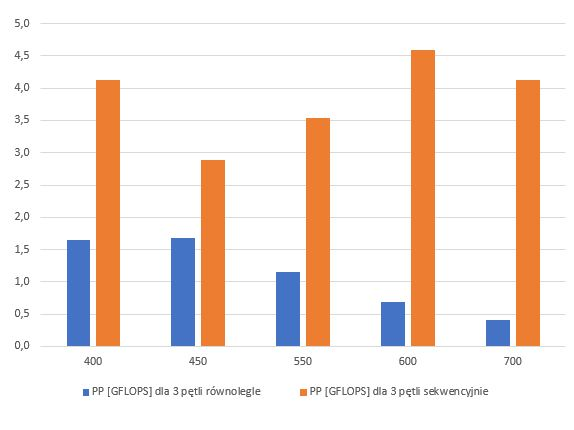
\includegraphics[width=0.7\textwidth]{PP.JPG}
	\caption{Porównanie PP w GFLOPS dla przetwarzania równoległego i sekwencyjnego}
\end{figure}

\newpage

\begin{figure}[h]
	\centering
	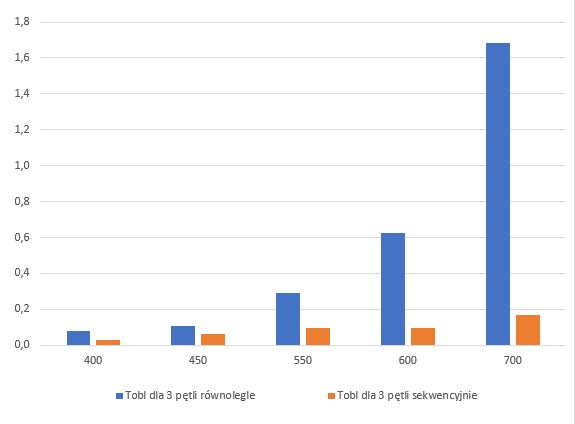
\includegraphics[width=0.7\textwidth]{Tobl.JPG}
	\caption{Porównanie Tobl w sekundach dla przetwarzania równoległego i sekwencyjnego}
\end{figure}

\begin{figure}[h]
	\centering
	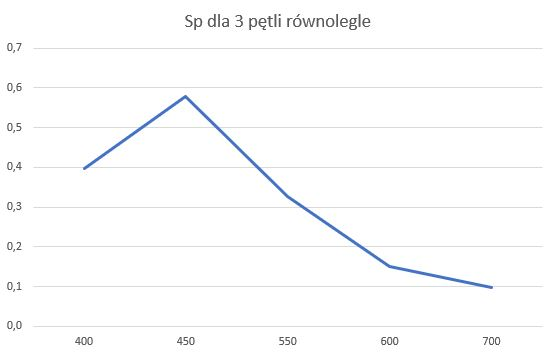
\includegraphics[width=0.7\textwidth]{SP.JPG}
	\caption{Zależność SP od wielkości instancji dla metody równoległej z 3 pętlami}
\end{figure}

\newpage

\section{Wnioski}
\subsection{Metoda 3 pętli}
\subsubsection*{Porównanie prędkości przetwarzania równoległego i sekwencyjnego}
Porównując prędkości przetwarzania można zauważyć, że metoda sekwencyjna cechuje się ogólnie
większymi wartościami PP, przy czym PP dla metody 3 pętli zaczyna znacząco spadać dla wielkości instancji
powyżej 450. Dzieje się tak dlatego, że dla $n\leq430$ zachowane są lokalność przestrzenna
i czasowa. Dla $596 \geq n \geq 430$ zachowana jest jedynie lokalność czasowa. Widać, że dla 
$n\geq600$ wartość PP spada jeszcze bardziej z powodu niezachowania lokalnośści czasowej 
i przestrzennej. Można to zaobserwować na wykresie na rysunku 6.\\
\\
Z tego samego powodu, jak widać na wykresie na rysunku 7., czas obliczeń dla metody równoległej
rośnie znacznie szybciej niż dla metody sekwencyjnej. Jest to szczególnie widoczne dla wartości
$n\geq600$, dla których nie są zachowane lokalność przestrzenna i czasowa.

\subsubsection*{Przyspieszenie przetwarzania równoległego}
Analizując wykres na rysunku 8. można zauważyć, że dla instancji o wielkości 450 występuje maksymalne
przyspieszenie. Nie jest to jednak zupełnie poprawne spostrzeżenie - rozdzielczość naszych pomiarów
nie pozwala nam tego dobrze zobrazować, jednak trzeba pamiętać, że tylko dla $n\leq430$ zachowana jest
lokalność przestrzenna. W rzeczywistości jest tak, że SP rośnie dla rozmiaru instancji do $n=430$,
właśnie ze względu na zachowaną lokalność przestrzenną. Nasępnie, co można zaobserwować na wykresie
przy naszej rozdzielczości pomiarów, przyspieszenie zaczyna spadać. Pamiętając o tym, że ta miara
bierze pod uwagę dwie różne wersje algorytmu (dla przetwarzania sekwencyjnego IKJ to najszybszy 
możliwy algorytm), można zauwazyć, że algorytm w wersji JKI wykonywany równolegle nie jest w 
stanie dorównać efektywności najszybszego algorytmu przetwarzania sekwencyjnego.

\subsubsection*{Wpływ utraty lokalności przestrzennej na efektywność przetwarzania}
Wielkość charakterystyczna, przy której metoda traci lokalność przestrzenną, wyznaczona ze wzoru (3), to n=430. Oznacza to, że dla instancji większych od
tej wartości procesor będzie zmuszony częściej przeglądać tablicę stron, zamiast korzystać z adresów w buforze translacji. 
Jeżeli popatrzymy na wskaźnik WBTBT to rzeczywiście widać, że od wartości rozmiaru instancji 450 liczba braków trafień 
do bufora translacji w stosunku do LIA gwałtownie rośnie i w momencie, gdy instancja ma rozmiar 700 wzrósł o 2 rzędy wielkości 
(liczba rzeczywistych braków trafień do bufora translacji jest przedstawiona w tablicy 2 w kolumnie BTBT - dla najmniejszej
instancji, kiedy zapewniona jest jeszcze lokalność przestrzenna liczba braku trafień do bufora translacji
leży w przedziale od 50 do 100 tys., natomiast w momencie przekroczenia wartości charakterystycznej, 
dla instancji o rozmiarze 550, kiedy ciągle zachowana jest lokalnośc czasowa, liczba ta mocno wzrasta 
osiągając wartość prawie 52 mln.). Koszty przeglądania tablicy stron są bardzo duże, więc utrata lokalności przestrzennej 
powoduje spadek efektywności przetwarzania, co ma odzwierciedlenie w miarach efektywności przedstawionych w tabeli (5). 
Dokładny wpływ utraty lokalności przestrzennej na miary efektywności jest przedstawiony w pozostałych paragrafach. 

\subsubsection*{Wpływ utraty lokalności czasowej na efektywność przetwarzania}
Korzystając ze wzoru (1) obliczyliśmy, że wartość charakterystyczna dla lokalności czasowej dla danej metody to 596. Dla większych 
instancji procesor przestaje znajdować potrzebne linie danych w pamięci podręcznej i musi je sprowadzać 
z pamięci RAM. Jest to proces bardzo kosztowny i negatywnie wpływa na efektywność i stąd na szybkość przetwarzania.
Z tabeli (5) widać, że dla instancji o rozmiarze 700 wskaźnik WBTL3 wzrósł o jeden cały rząd wielkości. Również patrząc na 
wskaźnik KPD można zauważyć duży wzrost liczby pobrań linii danych dla instancji, w której utracona lokalności czasowej. \\

Jednocześnie wskaźnik WDD, określający liczbę dostępów do danych w stosunku do LIA, wzrasta praktycznie niezauważalnie. 
Wynika to z faktu, że rozmiar instancji ma proporcjonalny wpływ zarówno na LIA jak i na liczbę dostępów do danych, więc stosunek 
tych dwóch wartości powinna zostać względnie stała i tak też jest w naszym przypadku. 

\subsubsection*{Średnia liczba instrukcji przypadająca na cykl prcesora}
Miary IPC1 i IPCS, oznaczające odpowiednio średnią liczbę instrukcji przypadającą na jeden cykl jednego procesora
oraz średnią liczbę instrukcji na cykl procesora dla całego systemu maleje wraz ze wzrostem rozmiaru instancji.
Mimo tego, że wraz ze wzrostem instancji LIA szybko wzrasta (dla 2x większej instancji LIA powinno być 4x większe) to 
liczba cykli procesora wzrasta dużo szybciej (wynika to z utraty lokalności przestrzennej i później lokalności czasowej, 
co zmusza procesor do wykonywania dodatkowych operacji w buforze translacji i pamięci podręcznej, co bardzo dobrze widać w 
tablicy 2, w kolumnach BTBT i BTL3). Jak widać z obliczeń przy zachowaniu lokalności przestrzennej i czasowej dla 
instancji o rozmiarze n=400 liczba instrukcji na cykl procesora wynosi 0.7552, natomiast dla instancji o rozmiarze n=700, 
gdzie nie była zachowa ani lokalnośc przestrzenna, ani czasowa liczba instrukcji spadła do 0.0884 na jeden cykl. Jest to 
obrzymi spadek średniej liczby instrukcji, przypadających na cykl zegara w jednym processie, jak i w całym systemie.

\subsubsection*{Miara kosztu synchronizacji}
Można zauważyć, że wskażnik miary kosztu synchronizacji dla rozpatrywanej metody jest bliski 0. Jako, że 
wskaźnik ten mierzy stosunek czasu, w którym wątki były bezczynne, do całkowitego czasu przetwarzania, oznacza
to, że praktycznie nie było momentów, w których wątki musiałyby czekać za zakończenie pracy przez inne wątki. 
Można więc stwierdzić, że zrównoleglenie przetwarzania jest korzystne pod względem całkowietj efektywności przetwarzania.\\
W jednym pomiarze wartość MKS przyjęła wartość ujemną, co może wynikać z faktu, że czas obliczeń (Tobl) był mierzony tylko 
dla operacji mnożenia macierzy, natomiast liczba cykli procesora była mierzona dla całego programu, łącznie z momentem
losowania wartości macierzy. We wzorze (12) w mianowniku od CCP (zależne od czasu obliczeń) odejmujemy CWP (wyznaczane 
względem liczby cykli procesora), więc biorąc pod uwagę obserwację opisaną powyżej, wartość mianownika może wyjść ujemna.synchronizacji

\subsection{Metoda 6 pętli}
\subsubsection*{Prędkość przetwarzania}
Prędkość przetwarzania dla instancji o stałym rozmiarze $n=1500$ jest, jak widać w tabeli (5), związana
z rozmiarem okna. Widać, że wraz ze wzrostem $r$ PP spada, a spadek ten jest szczegónie drastyczny kiedy następuje 
utrata lokalności czasowej.

\subsubsection*{Wpływ utraty lokalności przestrzennej na efektywność przetwarzania}
Rozmiar instancji, dla której utracona zostaje lokalność przestrzenna, został obliczony ze wzoru (4) i wynosi 362. 
Podobnie do wyników z metody 3 pętli, wzrost braku trafień do bufora translacji w stosunku do LIA można wyraźnie zauważyć
w tabeli (6) - dla instancji o rozmiarze 500 wartość ta wzrasta o dwa rzędy wielkości w stosunku do instancji o rozmiarze 
300, dla której lokalność przestrzenna była jeszcze zachowana.

\subsubsection*{Wpływ utraty lokalności czasowej na efektywność przetwarzania}
Lokalność czasowa zostaje utracona dla instancji większych od 707 (wartość obliczona ze wzoru (2)). Wpływ utraty tej lokalności
jest szczególnie widoczny, jeżeli spojrzymy na prędkość przetwarzania (PP spada z 2.28 Gflopsa do 0.92 GFlopsa). Jest to również
widoczne w tabeli (3) w kolumnie LCP.\\

Jak widać w tabeli (3) ilość liczby dostępów do pamięci jest praktycznie stała i nie powinno to budzić większych wątpliwości, ponieważ
rozmiar instancji jest stały i niezależnie od sposobu wykonania wszystkich obliczeń (czyli rozmiaru okna $r$). Zmianę widać dopiero przy 
zmianie wielkości instancji na 2000 - LDP wzrosło wtedy ponad dwukrotnie.

\subsubsection*{Miara kosztu synchronizacji}
W tym przypadku, podobnie jak dla jednej instancji w metodzie 3 pętli, MKS przyjmuje
wartości ujemne. Dzieje się tak dlatego, że mamy tu do czynienia ze znacznie większymi instancjami,
więc i losowanie wartości dla macierzy, którego nie uwzględniamy w $Tobl$, ale które też
generuje dużo instrukcji assemblera, zajmuje znacznie więcej czasu.\\
Widać, że najdalej od zera jest wartość MKS dla $r=100$, co da się wytłumaczyć tym, że
$Tobl$ jest tu najmniejszy, a wielkość instancji jest taka sama jak dla innych wielkości
okna.\\
\\
Największe podejrzenia budzi liczba instrukcji kodu asemblera w pomiarach dla rozmiarów okna $r=300$ i
$r=750$, których jest mniej niż możnaby się spodziewać. Z tego powodu również miara WDD przyjmuje dla 
tych pomiarów dziwne wartości - wraz ze 'skokami' w ilości instrukcji assemblera, gwałtownie zmienia
się wartość WDD, która jest ilorazem LDP i LIA, gdzie LDP jest w dobrym przybliżeniu stałe 
dla wszystkich rozmiarów okna. Podobna anomalia dotyczy też miar IPC1 i IPCS. 
Z braku innych wyjaśnień tego zjawiska, skłaniamy się ku teorii błędów w pomiarach metody 6 pętli dla tych rozmiarów okna.
\end{document}